\chapter[PAM Generation and Demodulation]{PAM Generation and Demodulation}

\section*{Aim}
To set-up and implement circuits to carry out pulse amplitude modulation. To design demodulationg circuits to detect the message from pulse amplitude modulated wave.
\section*{Theory}
Pulse amplitude modulation is a kind of modulation technique in which analog message signal is sampled at constant frequency - \emph{carrier frequency}. A pulse of specified duration is used to sample the message signal. When the pulse is on, the message is sampled and when it is off no message is sampled. This is a basic step in the digitization of analog message signals. The circuits to be implemented in this experiment does a kind of natural sampling.\footnote{For more on natural sampling, refer Digital Transmission \cite{Tomasi}}.

Waveforms showing pulse carriers whose amplitude is modulated buy message is shown in Figure \ref{PAMmod}. A simple way to implement this is to allow the message to be fed as the input to a switch and the switch ON/OFF time is controlled by the pulses at sampling frequency.

The demodulation of PAM waveform can be implemented by using a lowpass filter which passes message signal frequenies but blocks the carrier signal.
\begin{figure}[h]
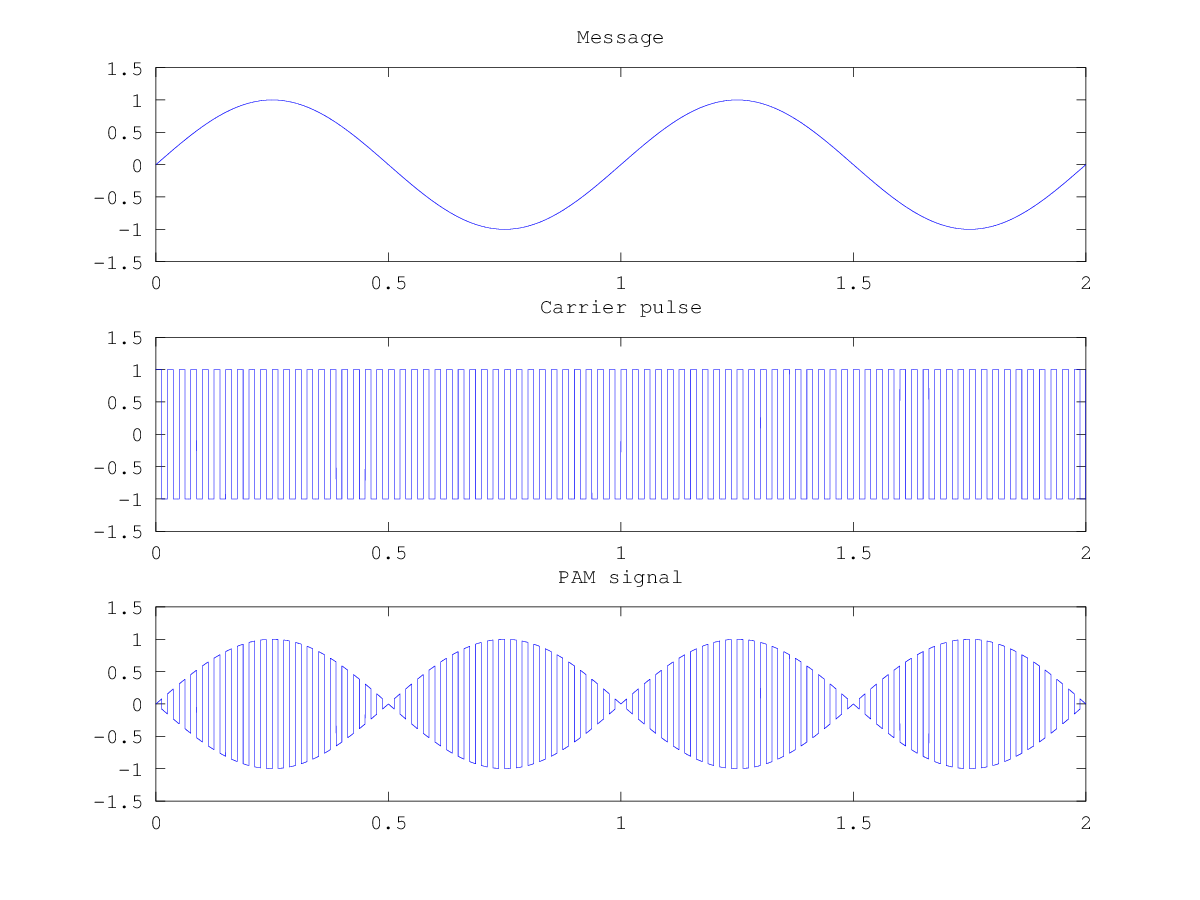
\includegraphics[width=\textwidth]{pam.png}
\caption{PAM modulation}
\label{PAMmod}
\end{figure}
\section*{Design}
\subsection*{PAM using transistor as a switch}
One technique to implement PAM is to use transistr in switching mode. The flow of current from collector to emitter in a bipolar junction transistor is controlled by the voltage at its base. 

\noindent Choose the transistor BC107.
\noindent Apply the message signal of frequency $fc < \ 1 \ kHz$ and amplitude $Em<\ 10\ V_{pp}$ at the collector.
\noindent Apply a carrier at the transistor base through a resistor $10 k\Omega$. The carrier pulse amplitude is set as $10 \ V_{pp}$ and frequency $f_c=\ 10 kHz$.

\subsection*{PAM using CMOS switching IC CD4016}
CD 4016 is a quad bilateral CMOS switching IC. The message signal is fed to any of the input terminals of the switch and the modulating pulse carrier is fed as the control signal for the switch. The PAM output will be available at the output terminal of the switch which is fed to the CRO via a load resistor of $10\ k\Omega$. Keep the message signal frequency to be $f_c=500 \ Hz$ and the switching pulse which is the carrier  be fed  from the TTL output of 10 kHz from a function generator.

\subsection*{Demodulation}
Demodulation is using a  $\pi$ RC filter.
\noindent Design the filter as per the equation for upper cut-off frequency of a low pass filter,
\begin{equation}
f_H=\frac{1}{2\pi R_dC_d}
\end{equation}
\begin{equation}
1\ kHz=\frac{1}{2\pi R_dC_d}
\end{equation}
\noindent Select $C_d=\ 0.01 \mu F$. Then $R_d=\ 16.1k\Omega$.
Choose $R_d=\ 15k\Omega \ or\ 22k\Omega$ standard resistor values.\\
\section*{Circuit Diagram}
\subsection*{Using transistor as a switch}
\subsection*{Using CMOS switching IC CD4016}

\section*{Procedure}
\section*{Observation}
\section*{Result}